\documentclass[12pt, letterpaper]{article}
\usepackage[utf8]{inputenc}
\usepackage{setspace}
\usepackage{subcaption} 
\usepackage{hyperref}
\usepackage{float}
\usepackage{url}
\usepackage{amsthm}
\usepackage{graphicx}
\usepackage{amssymb}
\usepackage{amsmath}
\usepackage[lastexercise]{exercise}
\usepackage{tikz}
\usetikzlibrary{matrix}
\graphicspath{{images/}} \newtheorem{definition}{Definition}[section] \newtheorem{theorem}{Theorem}[section]
\newtheorem{corollary}{Corollary}[theorem]
\newtheorem{lemma}[theorem]{Lemma}
\newcommand{\R}{\mathbb{R}}
\newcommand{\Z}{\mathbb{Z}}
\newcommand{\implies}{\Rightarrow}
\title{Morse Theory}
\author{Veronika Starodub \\ Miloš Vukadinović \\ Nikolay Ninov} \date{\today } 
\doublespacing
\begin{document} 
\maketitle

\begin{figure}[h]
    \centering
    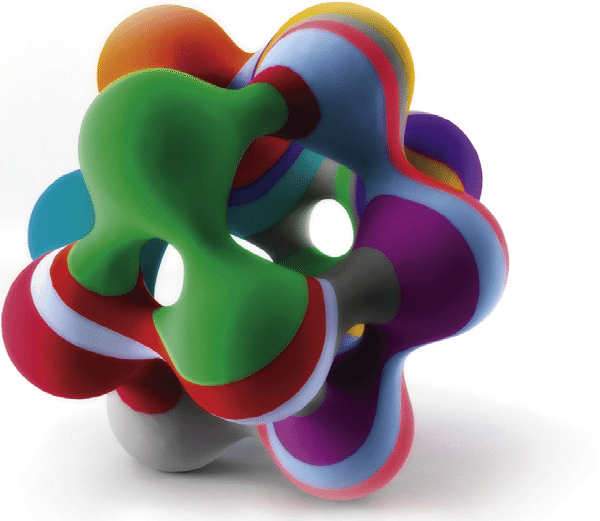
\includegraphics[width=0.50\textwidth]{cover}
\end{figure}
 
\tableofcontents
\section{Introduction}
\textbf{Ex.} Show that the function $f: S^2 \to \R, f(x,y,z) = z$ is a Morse function. \\

$f$ is smooth on $ S^2 $ since it extends to a smooth map on all of $\R^3$. We can map $R^3$ to $S^2$ with the stereographic projection two functions:\\
$
	\phi_1(x_1,x_2,x_3) = (\frac{x_1}{1-x_3}, \frac{x_2}{1-x_3} ) 
$
and
$
	\phi_2(y_1,y_2,y_3) = (\frac{y_1}{1+y_3},\frac{y_2}{1+y_3})
$\\
Therefore, to get $S^2 \to R^3$ we can take $\phi_1^{-1}$ and $\phi_2^{-1}$ \\
$
	\phi_1^{-1}(x_1,x_2,x_3) = (\frac{2x_1}{x_1^2+x_2^2+1}, \frac{2x_2}{x_1^2+x_2^2+1}, \frac{x_1^2+x_2^2-1}{x_1^2+x_2^2+1})
$\\
$
	\phi_1^{-1}(y_1,y_2,y_3) = (\frac{2y_1}{y_1^2+y_2^2+1}, \frac{2y_2}{y_1^2+y_2^2+1}, \frac{1-y_1^2+y_2^2}{y_1^2+y_2^2+1})
$\\
Then, we take $g_1 = f \circ \phi_1^{-1}$ and $g_2 = f \circ \phi_2^{-1}$ \\
$
	g_1(x,y) =  \frac{x^2+y^2-1}{x^2+y^2+1}
$
and
$
	g_2(x,y) = \frac{1-x^2+y^2}{x^2+y^2+1}
$ \\
Now, we can compute jacobian of $g_1$ and $g_2$, find critical points, and check that determinant of hessian matrix is non-zero. \\
$
	\nabla g_1(x,y,z) = 0$ iff $(x,y,z) = (0,0,-1)
$\\
$
	\nabla g_2(x,y,z) = 0$ iff $ (x,y,z) = (0,0,1)
$
We have two critical points, and now we compute the hessian at them.\\
$
	H(g_1) = \begin{bmatrix} 4 & 0 \\ 0 & 4 \end{bmatrix}
	\implies \det(H(g_1)) = 16
$\\
$
	H(g_2) = \begin{bmatrix} -4 & 0 \\ 0 & -4 \end{bmatrix}
	\implies \det(H(g_2)) =  16

$\\ 

Both critical points are non-degenerate, therefore $f$ is a Morse function.$\blacksquare$

\end{document}
